We now want to use the algorithm from the previous section to compute the spectral density of a unitary matrix~$U$. In order to assess the results, we need to compare the computed spectral density with the theoretical one. The problem is that the spectral density we defined applies to the real line, while the eigenvalues of a unitary matrix lie on the unit circle in the complex plane. To overcome this, we need to transform it a little first.

\section{Transformation of the Spectral Density for Comparison}

The exact spectral density at a point $x$ on the real line is given by
\[
\phi(x) = \sum_{i=1}^n \delta(x - \lambda_i),
\]
where $\delta$ is the Dirac delta function. For a regularized, smoothed delta function, one simply evaluates the regularization function at $x - \lambda_i$ for all $i$ and sums the result. We use Gaussian regularization in our implementation, with the Gaussian function defined as
\[
    g_\sigma(x) = \frac{1}{\sqrt{2\pi} \sigma} e^{-\frac{x^2}{2\sigma^2}},
\]
where $\sigma$ is the standard deviation of the Gaussian. This $\sigma$ is often called the \emph{target resolution} \cite{linsaadyang14}; the smaller it is, the higher the resolution of the spectral density. We need to balance high resolution for exactness with easier approximation for larger $\sigma$.
Then we replace the Dirac delta function in the spectral density with the Gaussian regularization function:
\[
    \phi_\sigma(x) := \sum_{i=1}^n g_\sigma(x - \lambda_i).
\]


However, we defined the spectral density only on the real line, while the eigenvalues of a unitary matrix lie on the unit circle. To be able to evaluate $\phi_\sigma(z)$ for $z \in \C$, we use the inverse Cayley transform $\varphi^{-1}(z) = i\frac{1 - z}{1 + z}$, which maps $z \in \mathbb{S}^1$ to $x \in \R$, and evaluate $\phi_\sigma(\varphi^{-1}(z))$. According to the standard change-of-variables formula for probability densities, this requires multiplying by the Jacobian determinant to ensure correct normalization:
\[
    \hat{\phi}_\sigma(z) = \phi_\sigma(\varphi^{-1}(z)) \, \frac{(\varphi^{-1}(z))^2 + 1}{2} = \sum_{i=1}^n g_\sigma(\varphi^{-1}(z) - \lambda_i) \, \frac{(\varphi^{-1}(z))^2 + 1}{2}.
\]
An exact computation for the Jacobian determinant is found in the appendix.

Before we can plot the spectral density of a unitary matrix $U$ on the unit circle, we need to consider which random unitary matrices to use for our numerical experiments. The choice of random unitary matrices is crucial, as it affects the distribution of eigenvalues and thus the spectral density we want to compute.

\section{The Choice of Random Unitary Matrices}

When generating random unitary matrices for numerical experiments, it is important to ensure that their eigenvalues are distributed uniformly on the unit circle, as predicted by random matrix theory~\cite{mezzadri2007}. A common approach is to generate a random complex matrix $A$ with independent standard normal entries and then construct a unitary matrix from $A$ using either the QR decomposition or the singular value decomposition (SVD). In the QR approach, $A$ is factored as $A = QR$, where $Q$ is unitary and $R$ is upper triangular. The matrix $Q$ is then used as the random unitary matrix. In the SVD approach, $A$ is factored as $A = U \Sigma V^*$, and either $U$ or $V$ (both unitary) can be used as a random unitary matrix.
Although both methods produce unitary matrices, their statistical properties differ.
The SVD-based approach yields unitary matrices whose eigenvalues are uniformly distributed on the unit circle,
matching the theoretical prediction for random unitary matrices (the so-called Haar measure)~\cite{mezzadri2007}.
In contrast, the QR-based approach does not generally produce a uniform distribution of eigenvalues on the unit circle. This distinction is important for applications where the spectral properties of random unitary matrices play a central role, such as in the study of spectral densities.

\begin{figure}[H]
    \centering
    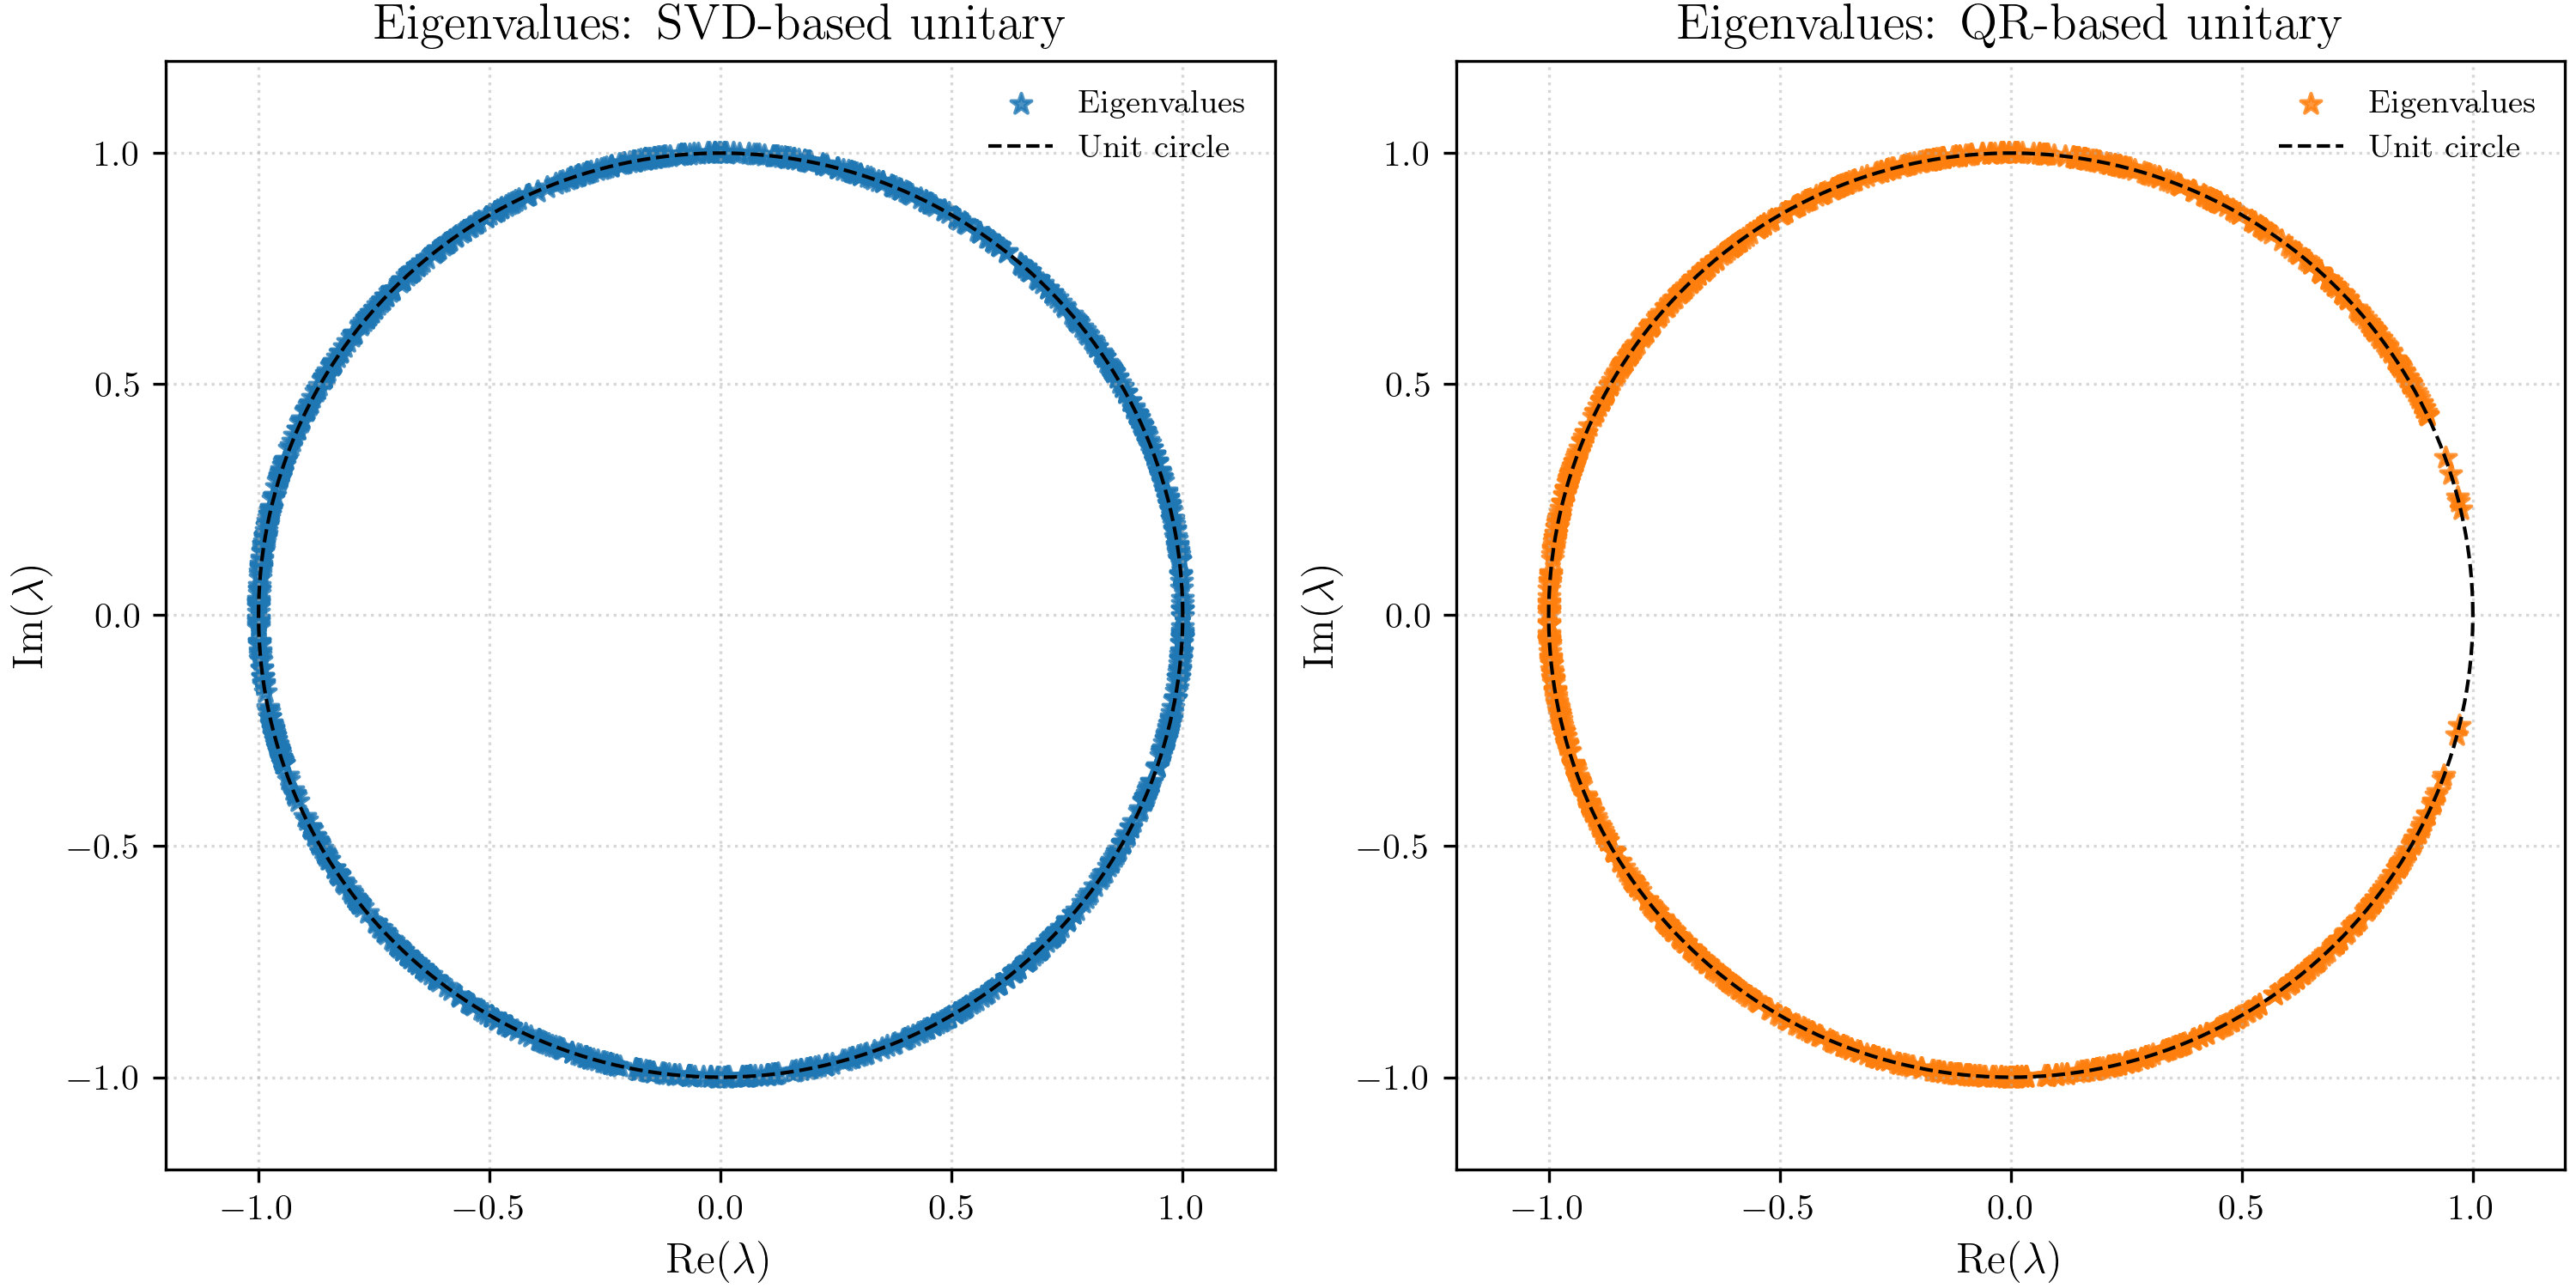
\includegraphics[width=1\textwidth]{Graphics/eigenvalue_comparison.png}
    \caption{Eigenvalue distributions of random unitary matrices generated via SVD and QR.}
    \label{fig:eigenvalue-comparison}
\end{figure}

We can now compare the spectral density of a SVD-based random unitary matrix $U$ with that of a QR-based random unitary matrix $Q$. We also show how the $\sigma$ influences the plots.

\begin{figure}[H]
    \centering
    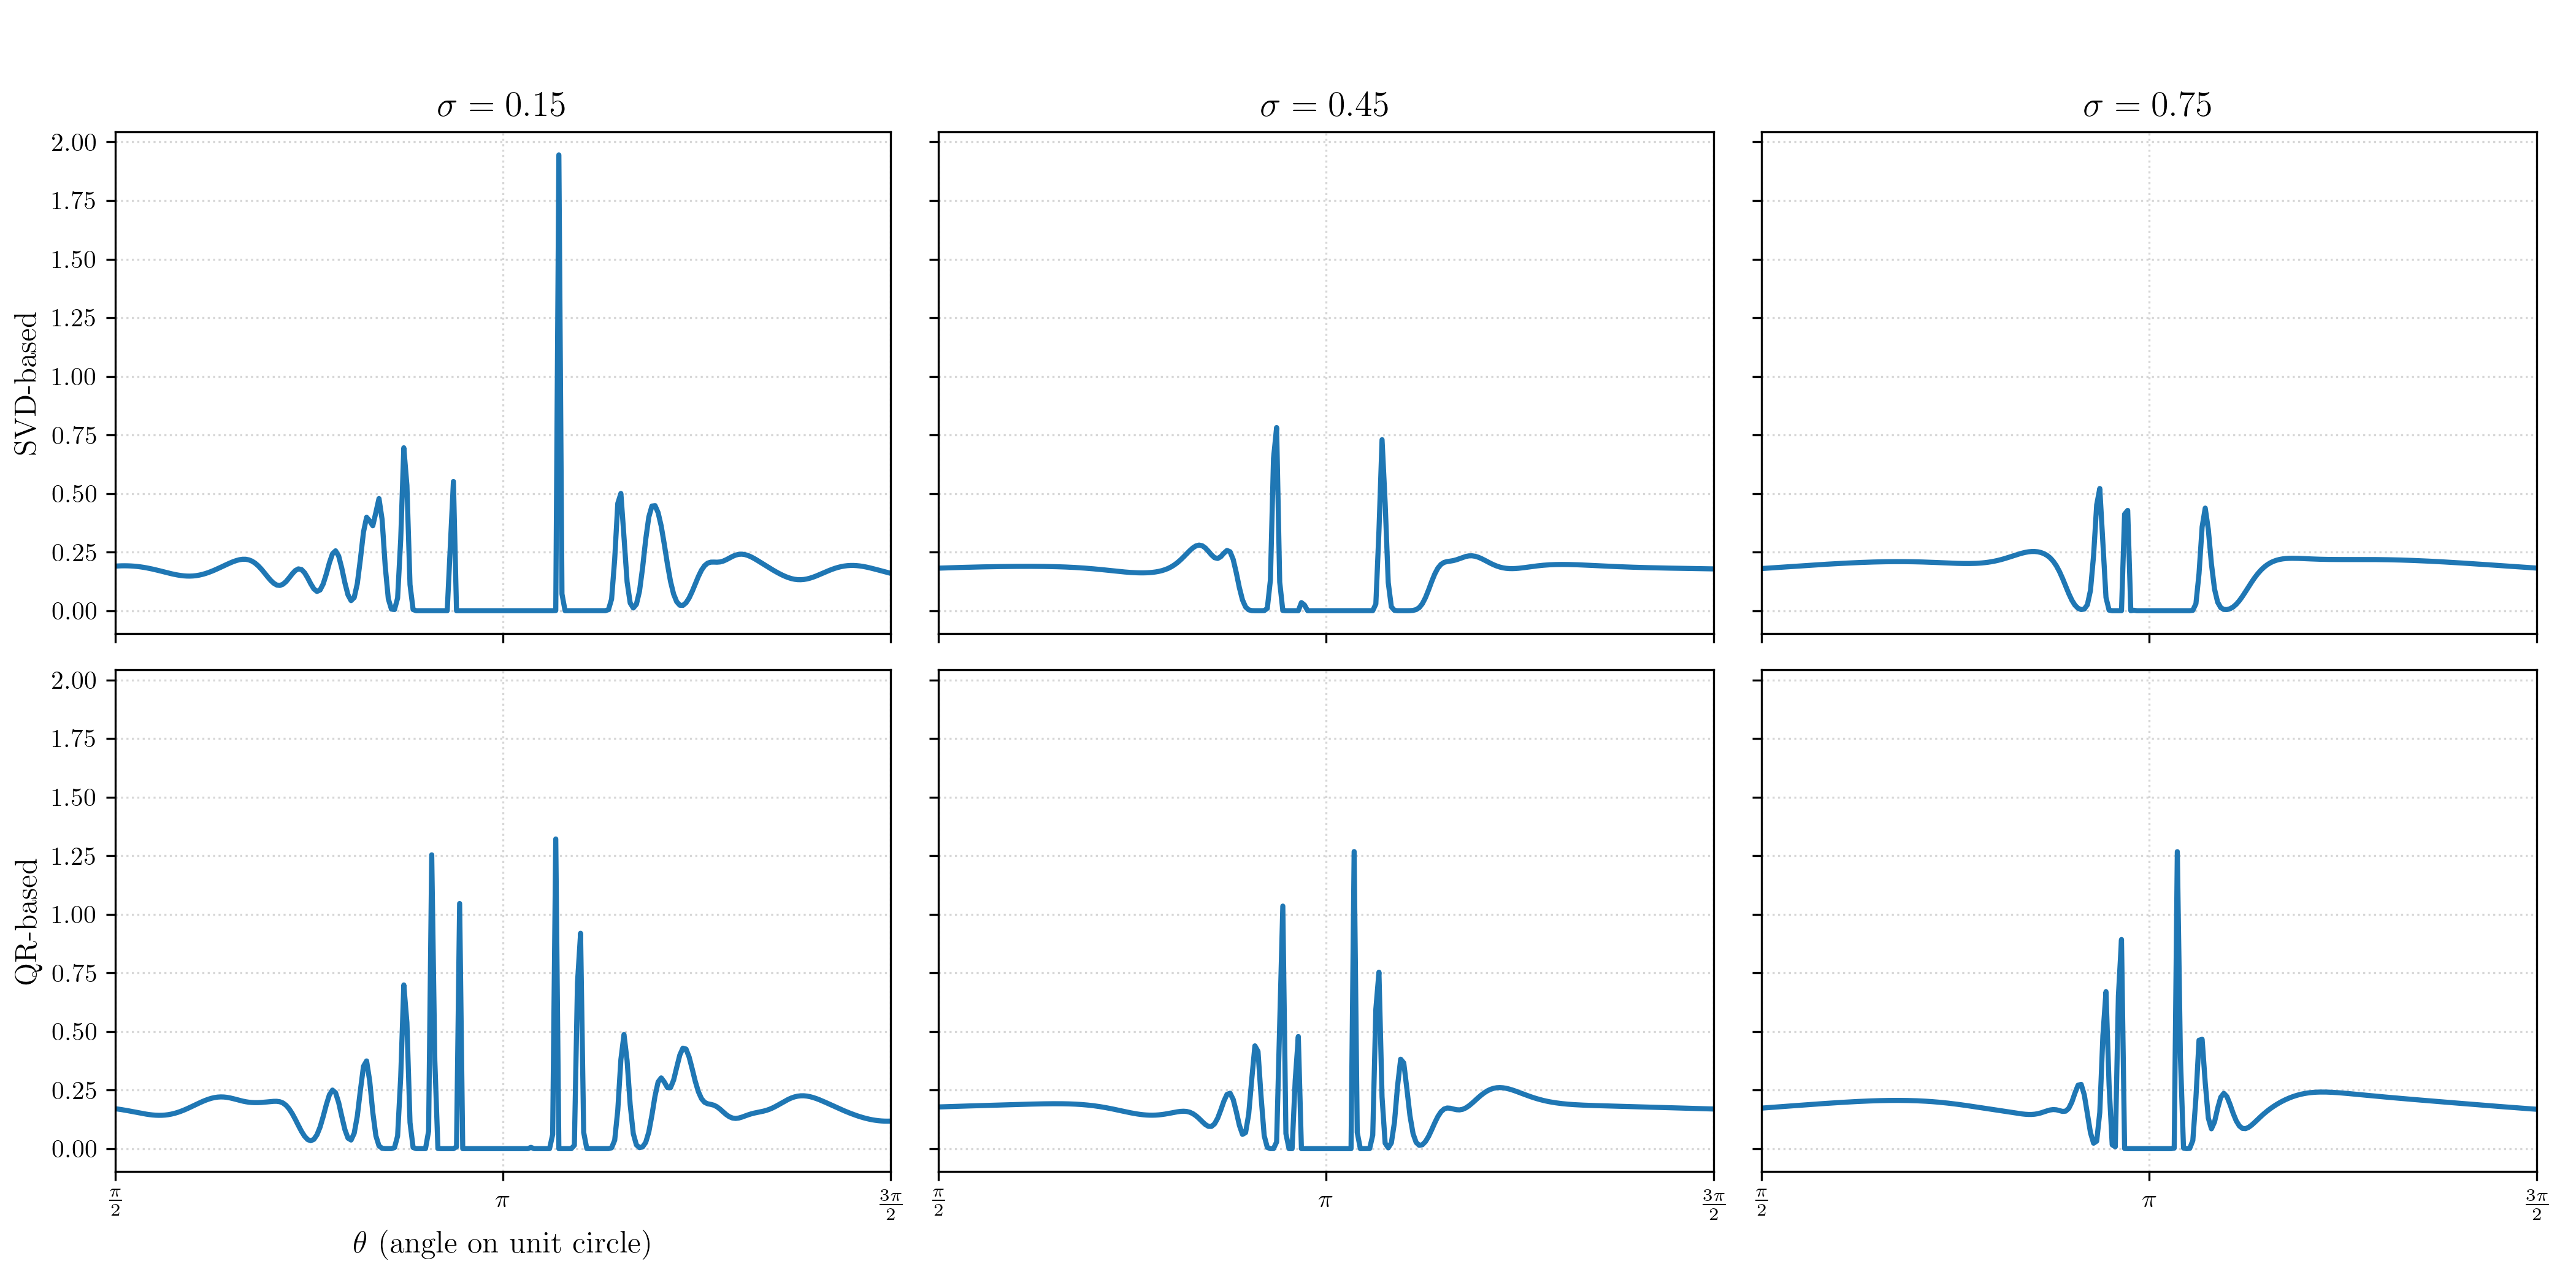
\includegraphics[width=1\textwidth]{Graphics/compare_svd_qr_spectral_density.png}
    \caption{Regularized spectral density of random unitary matrices generated via SVD and QR for varying $\sigma$.}
    \label{fig:spectral_density_comparison}
\end{figure}

It is evident, that a bigger $\sigma$ leads to a smoother spectral density but at the cost of losing information, while a smaller $\sigma$ captures more fine-grained features. This behavior is consistent across both SVD-based and QR-based random unitary matrices.